% A (minimal) template for problem sets and solutions using the exam document class

% Organization:
%% Define new commands, macros, etc. in macros.tex
%% Anything that you would put before \begin{document} should go in prelude.tex

%% For multiple psets, each should get its own file to \input into main with a \section{}
\documentclass[answers]{exam}
\qformat{}

\usepackage{cancel}
\usepackage{amsmath}
\usepackage{amsthm}
\usepackage{amsfonts}
\usepackage{mathtools}
\usepackage{amssymb}
\usepackage{mathrsfs}
\usepackage{graphicx}
\usepackage{enumitem}
\renewcommand{\qedsymbol}{$\blacksquare$}

\newcommand{\R}{\mathbb{R}}
\newcommand{\C}{\mathbb{C}}
\newcommand{\Z}{\mathbb{Z}}
\newcommand{\N}{\mathbb{N}}
\newcommand\tab[1][1cm]{\hspace*{#1}}
\newcommand{\K}{\mathbb{K}}
\newcommand{\zero}{\mathbb{O}}
\begin{document}

\title{Fourier Analysis and Wavelets\\Homework 2}
\author{Francisco Jose Castillo Carrasco}
\date{\today}
\maketitle

%% \union - Example: \union{j \in J}{A_j}
\newcommand{\union}[2]{\underset{#1}\bigcup #2}

%% \inter - like \union, but with \bigcap
\newcommand{\inter}[2]{\underset{#1}\bigcap #2}

%% Content goes here

\section*{Problem 10}
\begin{questions}

\question{
}
\begin{solution}

\end{solution}

\end{questions}

\newpage
\section*{Problem 18}
\begin{questions}

\question{Let $f$ and $g$ be $2\pi$-periodic, piecewise smooth functions having Fourier series $f(x)=\sum_n\alpha_ne^{inx}$ and $g(x)=\sum_n\beta_ne^{inx}$, and define the convolution of $f$ and $g$ to be $f*g(x)=\frac{1}{2\pi}\int_{-\pi}^{\pi}f(t)g(x-t)dt$. Show that the complex form of the Fourier series for $f*g$ is 
\begin{align*}
f*g(x)=\sum_{n=-\infty}^{\infty}\alpha_n\beta_ne^{inx}~.
\end{align*}
}
\begin{solution}
To prove the result is rather simple, it suffices with plugging in the Fourier series of the different functions in the convolution definition and operate:
\begin{align*}
f*g(x)=\frac{1}{2\pi}\int_{-\pi}^{\pi}f(t)g(x-t)dt&=\frac{1}{2\pi}\int_{-\pi}^{\pi}\sum_n\alpha_ne^{int}\sum_m\beta_me^{im(x-t)}dt\\
&=\frac{1}{2\pi}\sum_n\sum_m\alpha_n\beta_me^{imx}\int_{-\pi}^{\pi}e^{int}e^{-imt}dt\\
&=\frac{1}{2\pi}\sum_n\sum_m\alpha_n\beta_me^{imx}\int_{-\pi}^{\pi}e^{i(n-m)t}dt.
\end{align*}
We know that the set of complex exponentials is orthogonal. Hence, the integral is zero if $n\neq m$ and $2\pi$ if $n=m$. Therefore,
\begin{align*}
f*g(x)&=\frac{1}{2\pi}\sum_n\sum_m\alpha_n\beta_me^{imx}\int_{-\pi}^{\pi}e^{i(n-m)t}dt\\
&=\sum_n\alpha_n\beta_ne^{inx},
\end{align*}
and the result is proved.
\end{solution}
\end{questions}

\newpage
\section*{Problem 23}
\begin{questions}

\question{Sketch two periods of the pointwise limit of the Fourier series for each of the following functions. State wether or not each function's Fourier series converges uniformly. \newline

(e) $f(x)=\cos(x)+|\cos(x)|$, $-\pi\leq x\leq \pi$.
}
\begin{solution}
As we can see in the next figure, the function $f$ is continuous, piecewise smooth and $2\pi$-periodic. Hence, by \textsl{Theorem 1.30}, the Fourier Series for this function converges uniformly to it.
\end{solution}
\end{questions}


\section*{Problem 34}
\begin{questions}

\question{Consider the function
\begin{align*}
f(x)=e^{-x^2/10}\left(\cos 2x+2\sin 4x+0.4\cos 2x\cos 40x\right)~.
\end{align*}
For what values of $n$ would you expect the Fourier coefficients $a(n)$ and $b(n)$ to be significant. Why? Compute the $a(n)$ and $b(n)$ through $n=50$ and see if you are right. Plot the partial Fourier series through $n=6$ and compare with the plot of the original $f(x0$.
}
\begin{solution}

\end{solution}
\end{questions}

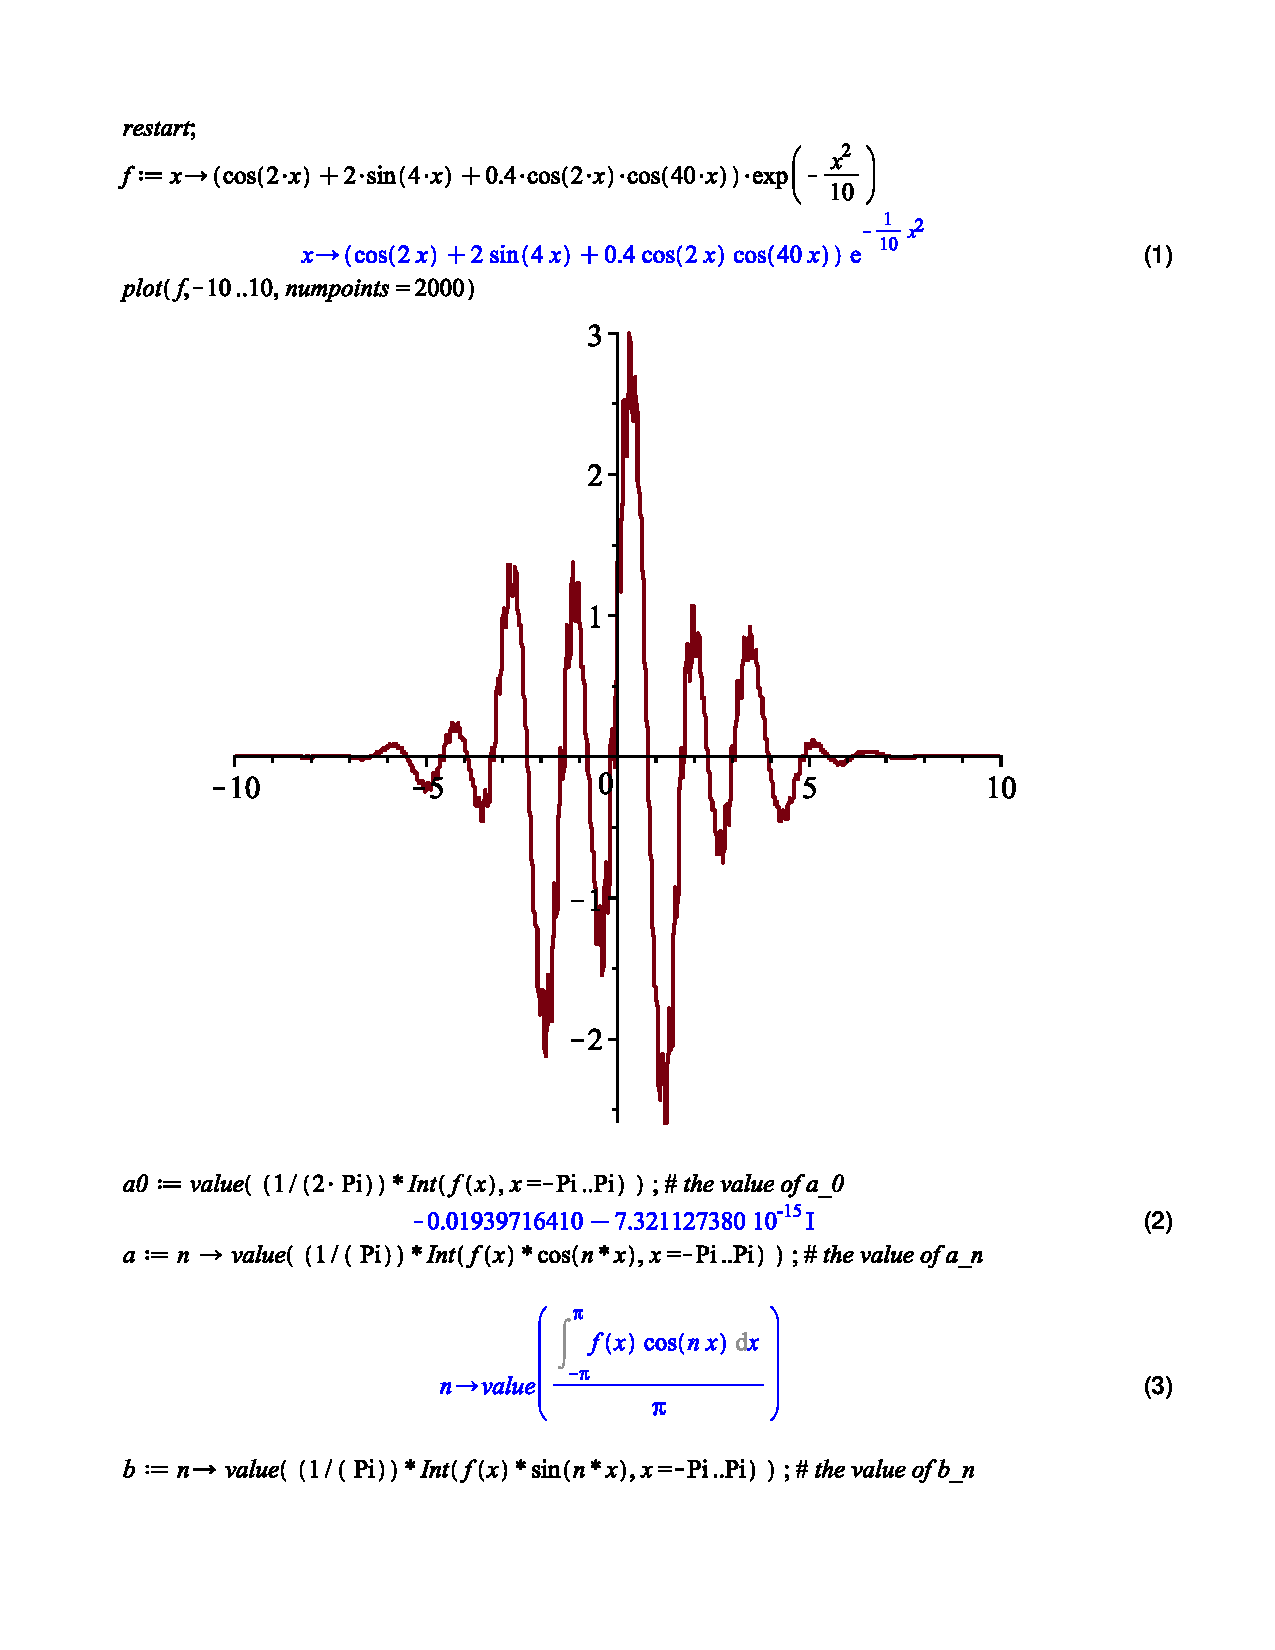
\includepdf[pages=-]{problem34}
\section*{Problem 35}
\begin{questions}

\question{Consider the function
\begin{align*}
g(x)=e^{-x^2/8}\left(\cos 2x+2\sin 4x+0.4\cos 2x\cos 10x\right)~.
\end{align*}
Compute the partial Fourier series through $N=25$. Throw away any coefficients that are smaller than $0.01$ in absolute value. Plot the resulting series and compare with the original function $g(x)$. Try experimenting with different tolerances.
}
\begin{solution}

\end{solution}
\end{questions}

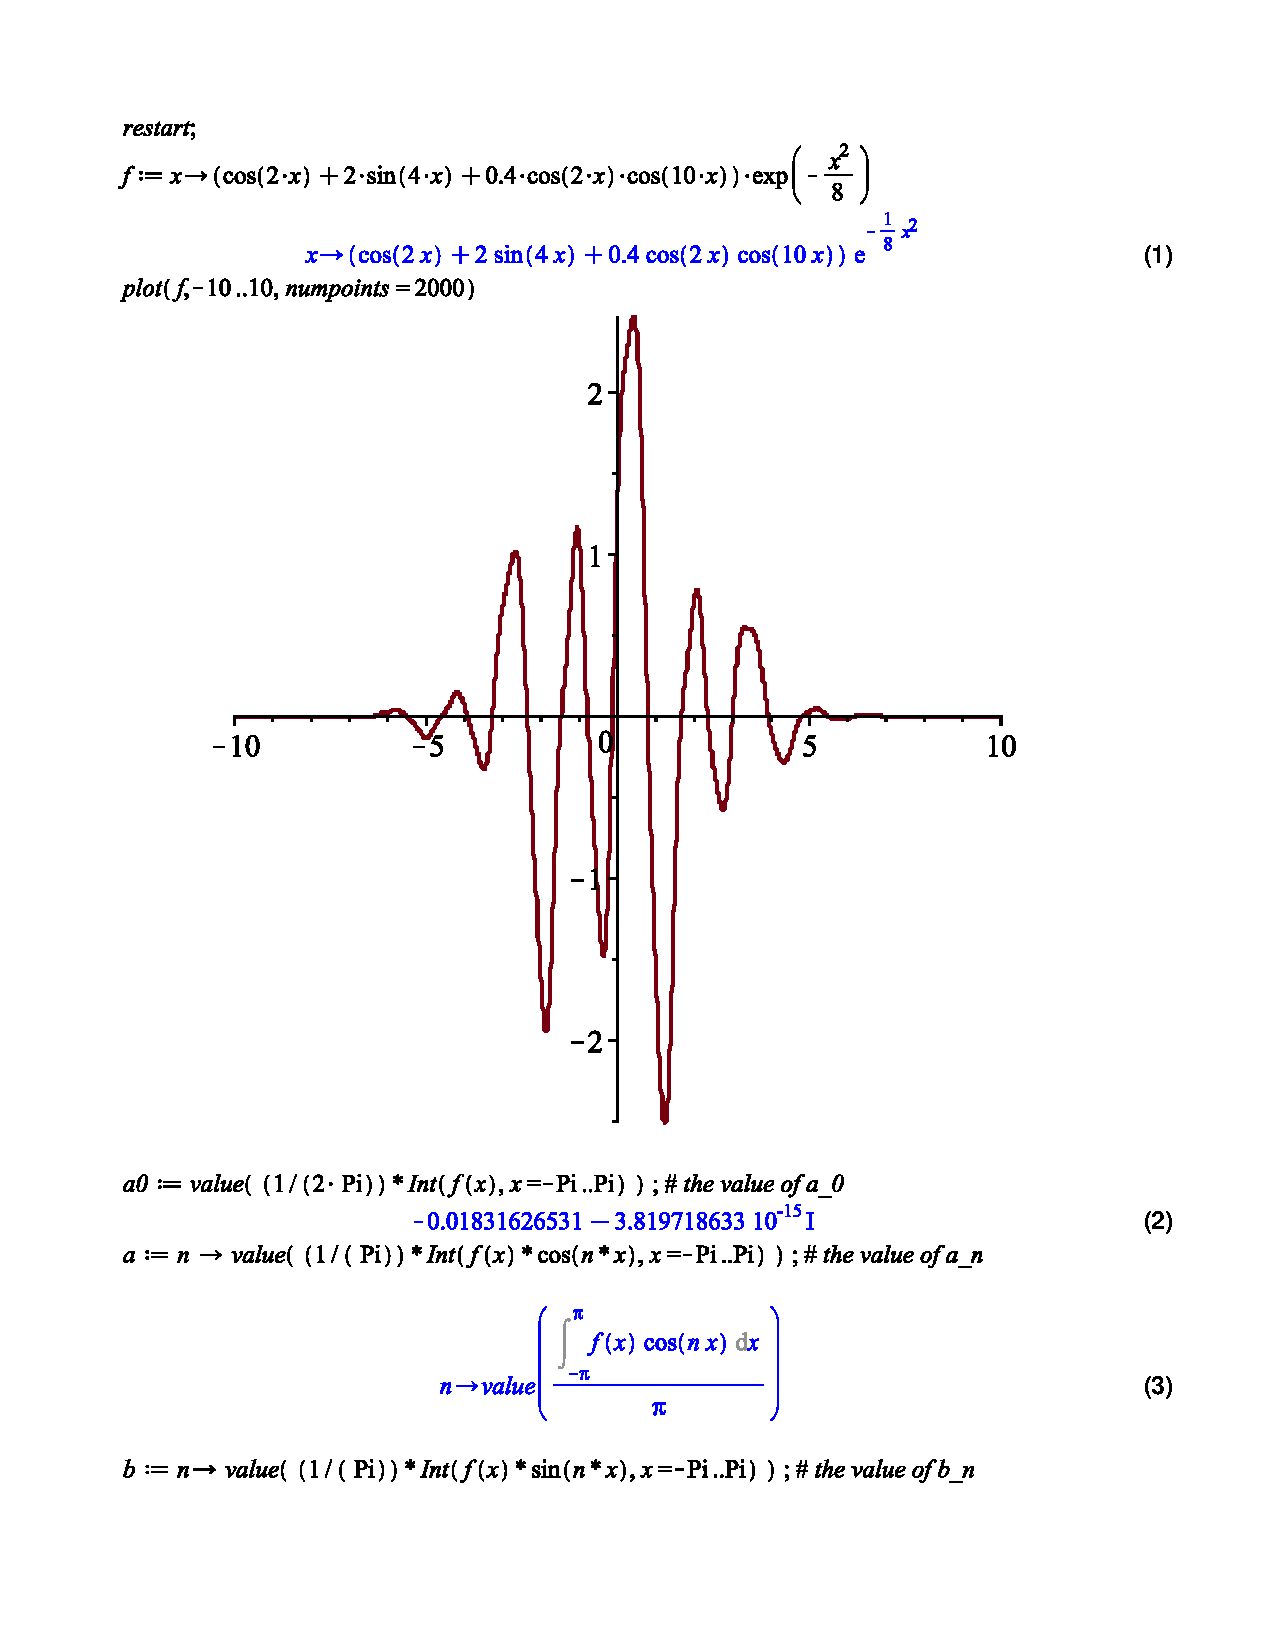
\includepdf[pages=-]{problem35}
\end{document}
